\documentclass[14pt]{article}
\usepackage{amsmath}
\usepackage{listings} % For writing code see http://ctan.org/pkg/listings
\usepackage{graphicx}
\usepackage{float}
\usepackage[margin=1.0in]{geometry}
\usepackage{hyperref}
\usepackage{fancyhdr}

\pagestyle{fancy}

\title{BFE high values on the coefficients with high order $l$}
\author{Nico Garavito-Camargo}


\begin{document}
\maketitle

\section{A review of the BFE formalism:}

In this document we will follow the notation presented Lowing11. Table
\ref{tab:conversion} shows the conversion between the Hernquist02 and Lowing11
notation.

\begin{table}[h]
  \centering
  \begin{tabular}{c  c}
    \hline
    \hline
    Hernquist+92 notation & Lowing+11 notation \\
    \hline
    $A_{nlm}$ & $S_{nlm} cos\ m\phi + T_{nlm}sin\ m\phi $\\
    $I_{nl} = 1/\tilde{A}_{nl}$ & $1/\tilde{A}_{nl}$\\
    $K_{nl}$ & $K_{nl}$ \\
    $\tilde{\rho}_{nl}$ & $\rho_{nl}$\\
    $\tilde{\Phi}_{nl}$ & $\Phi_{nl}$\\
    \hline
    \hline
  \end{tabular}
  \caption{Notation conversion between Hernquist92 and Lowing11
  papers}\label{tab:conversion}
\end{table}



The main idea of the BFE formalism is to expand the potential and density in
angular and radial functions. 




\begin{equation}
    \rho(r, \theta, \phi) = \sum_{nlm} A_{nlm}\rho_{nlm}(r, \theta, \phi)
\end{equation}

\begin{equation}
    \Phi(r, \theta, \phi) = \sum_{nlm} A_{nlm}\Phi_{nlm}(r, \theta, \phi)
\end{equation}

Where both the radial and angular parts can be expressed independently as:


\begin{equation}
  \Phi_{nlm}(r) = - \dfrac{r^l}{r(1+r)^{2l+3}}C_{n}^{2l+3/2}(\xi)\sqrt{4\pi}
\end{equation}


\begin{equation}
  \rho_{nl}(r) = \dfrac{K_{nl}}{2\pi}\dfrac{r^l}{(1+r)^{2l+1}}C_{n}^{2l+3/2}(\xi)\sqrt{4\pi}
\end{equation}

Where $K_{nl}$ is defined as:
\begin{equation}
    K_{nl}=\dfrac{1}{2}n(n+4l+3) +(l+1)(2l+1)
\end{equation}

In real space the full expansion takes the form: 


\begin{equation}
  \rho(r, \theta, \phi) = \sum_{n} \sum_l \sum_m Y_{lm}(\theta) \rho_{nl}(r)
  \left[ S_{nlm} cos m\phi + T_{nlm} sin m \phi \right]
\end{equation}


\begin{equation}
  \Phi(r, \theta, \phi) = \sum_{n} \sum_l \sum_m Y_{lm}(\theta) \Phi_{nl}(r)
  \left[ S_{nlm} cos m\phi + T_{nlm} sin m \phi \right]
\end{equation}


The coefficients can be computed using the orthonormal properties of the
Spherical harmonics and the Ultraspherical polynomials this is:

\begin{equation}\label{eq:energy}
  I_{nlm}^{n'l'm'} = \int_V \rho_{nlm} \Phi_{n'l'm'}^* = \tilde{A}_{nl} \delta_{nn'}
  \delta_{ll'} \delta_{mm'} 
\end{equation}

Where $\tilde{A}_{nl}$ is found to be:

\begin{equation}
    \tilde{A}_{nl} = - \frac{1}{K_{nl}}\frac{2^{8l+6}}{4\pi}\frac{n!(n+2l+3/2)[\Gamma(2l+3/2)]^2}{\Gamma(n+4l+3)}
\end{equation}

With these results we can compute the total gravitational energy of the system
as:

\begin{equation}
  U = \int_V \rho(r)\Phi(r)^{*} = \int_v  \sum_{nlm} A_{nlm}^2 \rho_{nlm}(r,
  \theta, \phi) \phi_{nlm}(r, \theta, \phi) = \sum_{nlm}
  \frac{A_{n'l'm'}^2}{\tilde{A}_{nl}}
  \delta_{nn'}\delta_{ll'}\delta_{mm'} 
\end{equation}

\begin{equation}
  U = \sum_{nlm} \frac{A_{n'l'm'}^2}{\tilde{A}_{nl}} 
\end{equation}


\section{Test-example with a Hernquist halo:}


\begin{figure}[h]
  \centering
  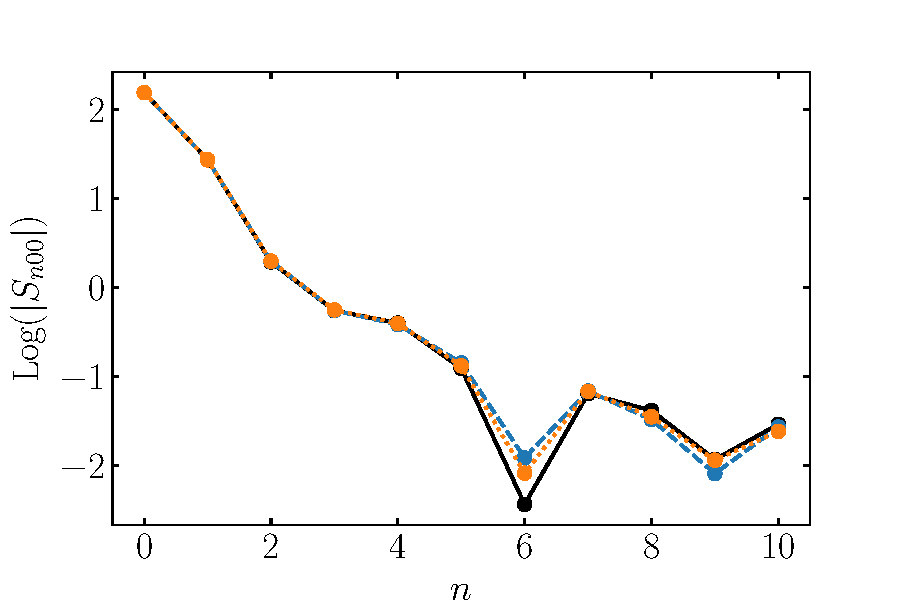
\includegraphics[scale=0.5]{../code/S_n_henrquist.pdf}
  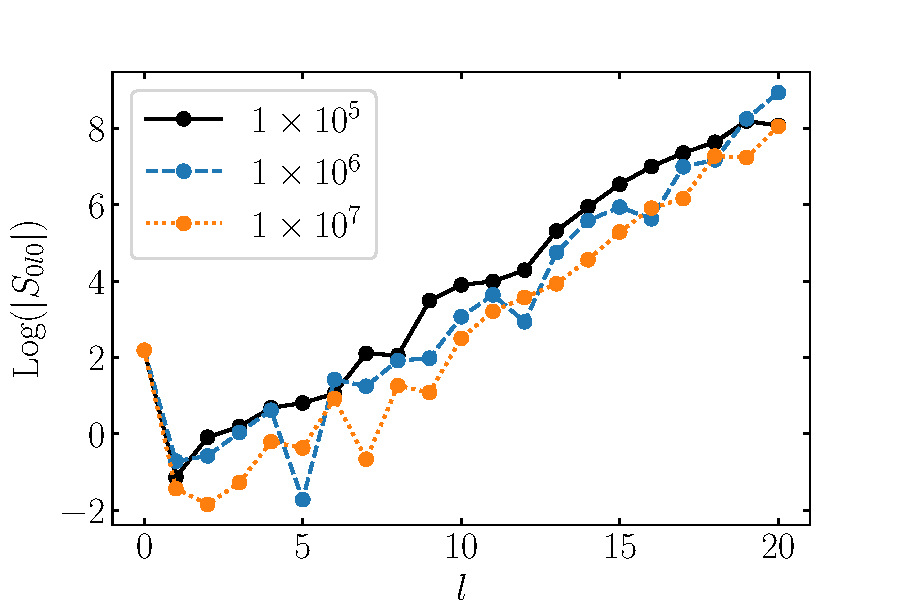
\includegraphics[scale=0.5]{../code/S_l_henrquist.pdf}
  \caption{Hernquist halos}

\end{figure}


\begin{figure}[h]
  \centering
  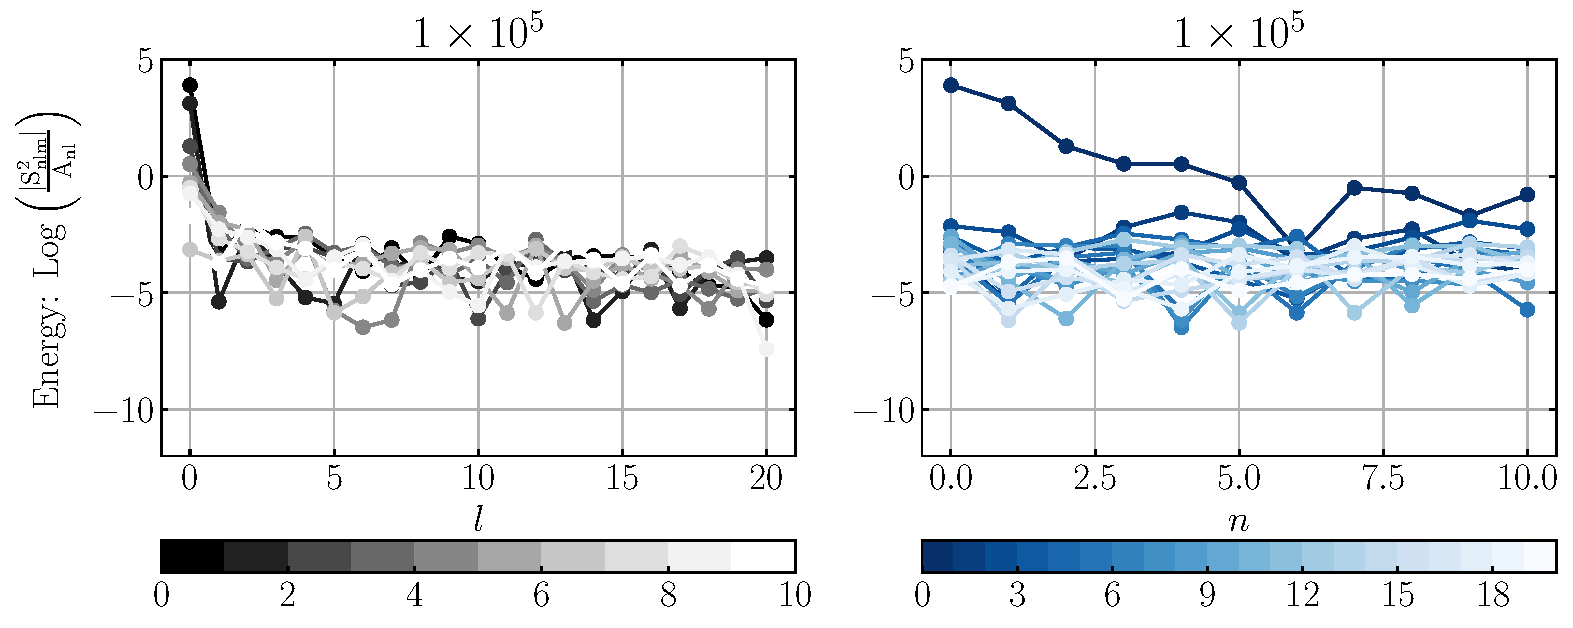
\includegraphics[scale=0.5]{../code/energy_terms_hern_a_40_1E5.pdf}
  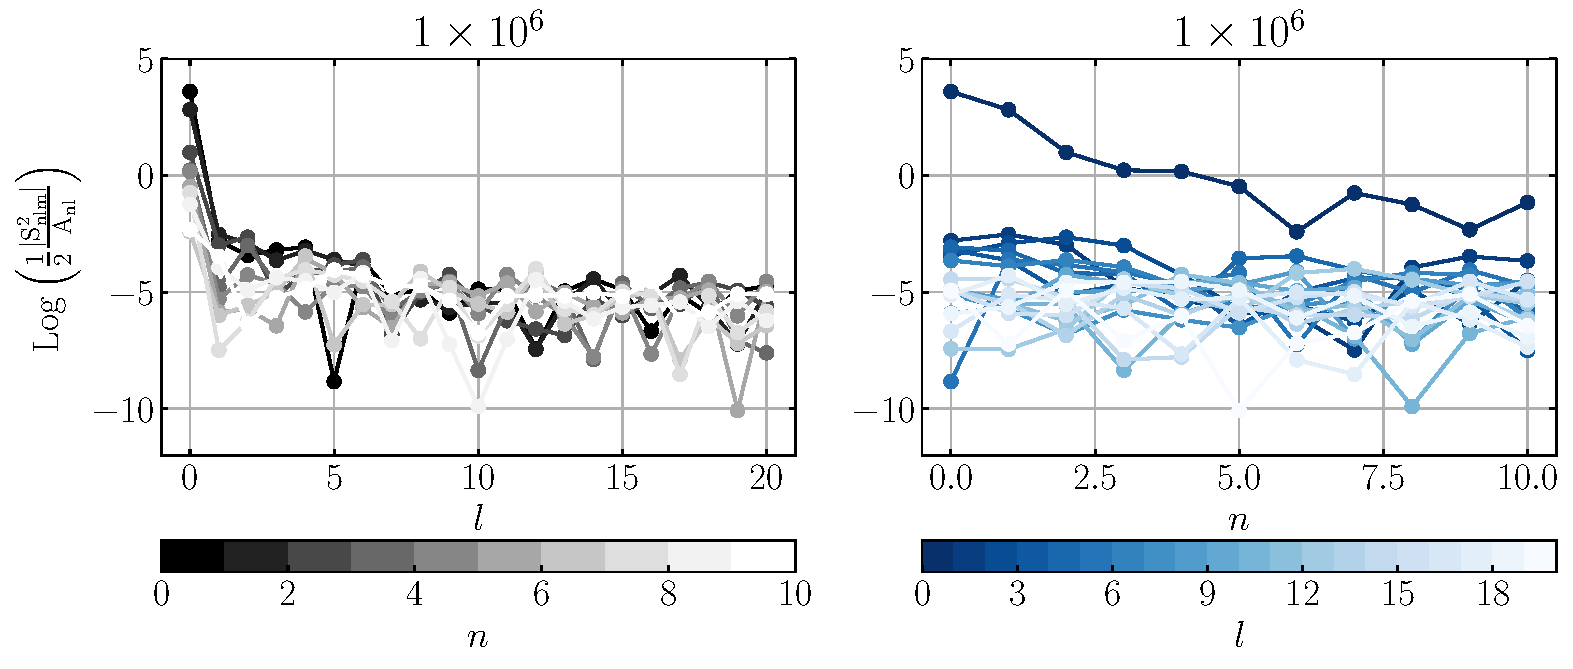
\includegraphics[scale=0.5]{../code/energy_terms_hern_a_40_1E6.pdf}
  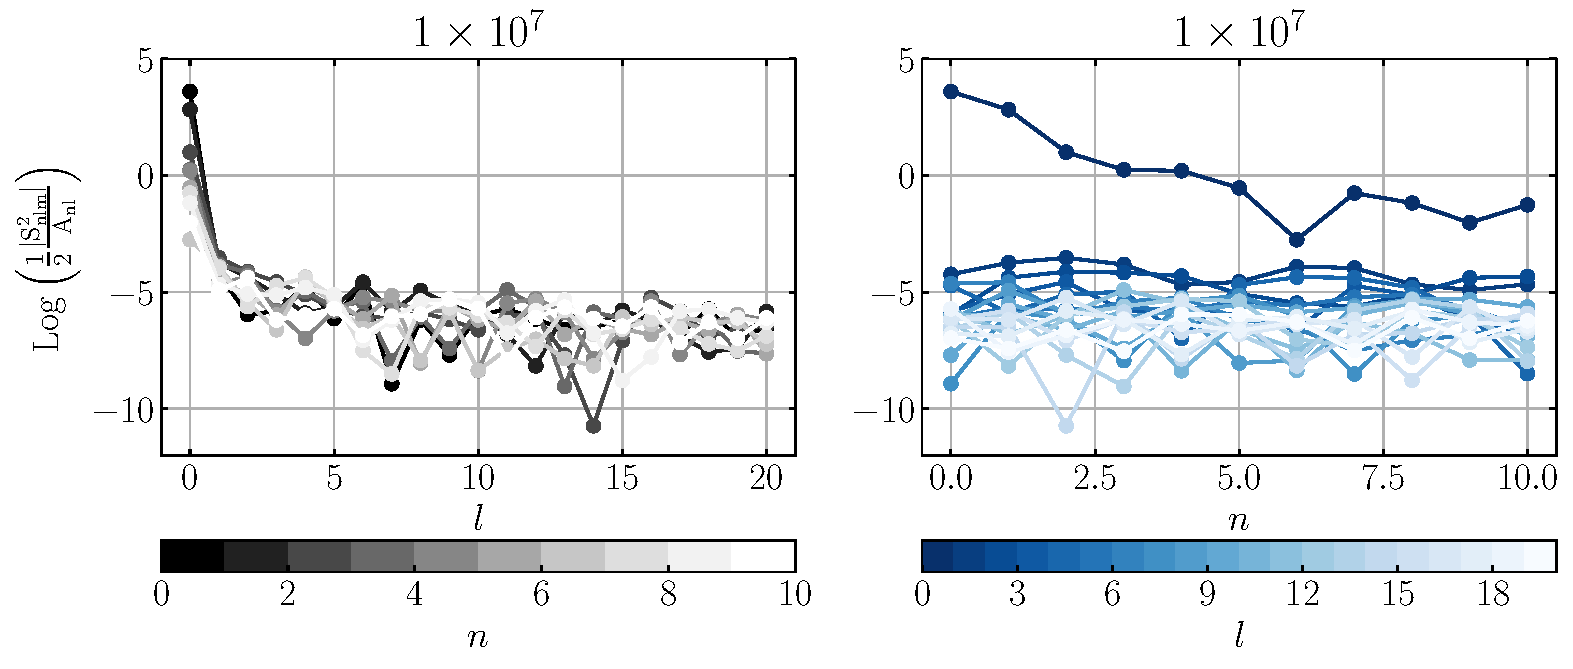
\includegraphics[scale=0.5]{../code/energy_terms_hern_a_40_1E7.pdf}
\end{figure}








\end{document}

